\documentclass[12pt]{article}
\usepackage[a4paper, left=30mm, right=20mm, top=20mm, bottom=20mm]{geometry}
\usepackage[utf8]{inputenc}
\usepackage[T2A]{fontenc}
\usepackage[russian]{babel}
\usepackage{amsmath, amssymb, amsthm}
\usepackage{graphicx}
\usepackage{hyperref}
\usepackage{mathrsfs}
\DeclareMathOperator{\SpanOp}{span}
\usepackage{booktabs}
\usepackage{algorithm}
\usepackage{float}
\usepackage{hyperref}
\usepackage{algpseudocode}
\usepackage{caption}
\usepackage{subcaption}
\usepackage{listings}
\usepackage{tabularx}
\usepackage{xcolor}
\usepackage{csquotes}
\usepackage[backend=biber,style=gost-numeric,sorting=none]{biblatex}

% Настройки для листингов кода
\lstset{
	language=Python,
	basicstyle=\ttfamily\small,
	keywordstyle=\color{blue},
	commentstyle=\color{gray},
	stringstyle=\color{green},
	numbers=left,
	numberstyle=\tiny\color{gray},
	stepnumber=1,
	numbersep=5pt,
	backgroundcolor=\color{white},
	frame=single,
	tabsize=4,
	captionpos=b,
	breaklines=true,
	breakatwhitespace=false,
	showspaces=false,
	showstringspaces=false,
	inputencoding=utf8,
	extendedchars=true,
	literate={а}{{\selectfont\char224}}1
	{б}{{\selectfont\char225}}1
	{в}{{\selectfont\char226}}1
	{г}{{\selectfont\char227}}1
	{д}{{\selectfont\char228}}1
	{е}{{\selectfont\char229}}1
	{ё}{{\"e}}1
	{ж}{{\selectfont\char230}}1
	{з}{{\selectfont\char231}}1
	{и}{{\selectfont\char232}}1
	{й}{{\selectfont\char233}}1
	{к}{{\selectfont\char234}}1
	{л}{{\selectfont\char235}}1
	{м}{{\selectfont\char236}}1
	{н}{{\selectfont\char237}}1
	{о}{{\selectfont\char238}}1
	{п}{{\selectfont\char239}}1
	{р}{{\selectfont\char240}}1
	{с}{{\selectfont\char241}}1
	{т}{{\selectfont\char242}}1
	{у}{{\selectfont\char243}}1
	{ф}{{\selectfont\char244}}1
	{х}{{\selectfont\char245}}1
	{ц}{{\selectfont\char246}}1
	{ч}{{\selectfont\char247}}1
	{ш}{{\selectfont\char248}}1
	{щ}{{\selectfont\char249}}1
	{ъ}{{\selectfont\char250}}1
	{ы}{{\selectfont\char251}}1
	{ь}{{\selectfont\char252}}1
	{э}{{\selectfont\char253}}1
	{ю}{{\selectfont\char254}}1
	{я}{{\selectfont\char255}}1
	{А}{{\selectfont\char192}}1
	{Б}{{\selectfont\char193}}1
	{В}{{\selectfont\char194}}1
	{Г}{{\selectfont\char195}}1
	{Д}{{\selectfont\char196}}1
	{Е}{{\selectfont\char197}}1
	{Ё}{{\"E}}1
	{Ж}{{\selectfont\char198}}1
	{З}{{\selectfont\char199}}1
	{И}{{\selectfont\char200}}1
	{Й}{{\selectfont\char201}}1
	{К}{{\selectfont\char202}}1
	{Л}{{\selectfont\char203}}1
	{М}{{\selectfont\char204}}1
	{Н}{{\selectfont\char205}}1
	{О}{{\selectfont\char206}}1
	{П}{{\selectfont\char207}}1
	{Р}{{\selectfont\char208}}1
	{С}{{\selectfont\char209}}1
	{Т}{{\selectfont\char210}}1
	{У}{{\selectfont\char211}}1
	{Ф}{{\selectfont\char212}}1
	{Х}{{\selectfont\char213}}1
	{Ц}{{\selectfont\char214}}1
	{Ч}{{\selectfont\char215}}1
	{Ш}{{\selectfont\char216}}1
	{Щ}{{\selectfont\char217}}1
	{Ъ}{{\selectfont\char218}}1
	{Ы}{{\selectfont\char219}}1
	{Ь}{{\selectfont\char220}}1
	{Э}{{\selectfont\char221}}1
	{Ю}{{\selectfont\char222}}1
	{Я}{{\selectfont\char223}}1
}

\addbibresource{references.bib}

\title{Универсальная аппроксимация с неограниченными активациями (ReLU)}
\author{Иванов Иван Иванович \\ Группа ПМИ-123}
\date{2024}

\newtheorem{theorem}{Теорема}
\newtheorem{lemma}{Лемма}
\newtheorem{definition}{Определение}
\newtheorem{corollary}{Следствие}
\newtheorem{proposition}{Предложение}
\newtheorem{remark}{Замечание}
\newtheorem{example}{Пример}

\DeclareMathOperator{\spn}{span}
\DeclareMathOperator{\supp}{supp}
\newcommand{\R}{\mathbb{R}}
\newcommand{\N}{\mathbb{N}}
\newcommand{\CC}{\mathcal{C}}  % Изменено с \C на \CC
\newcommand{\norm}[1]{\left\| #1 \right\|}
\DeclareUnicodeCharacter{221E}{\infty}  % Для символа бесконечности

\begin{document}
	
	\begin{titlepage}
		\centering
		
		Санкт-Петербургский государственный университет \\
		Прикладная математика, программирование и искусственный интеллект \\
		
		\vspace{4cm}
		
		Отчет по учебной практике 4 (научно-исследовательской работе) (семестр 4) \\
		Количественные оценки универсальной
		аппроксимации ReLU-сетями:
		скорость приближения, глубина и минимальная ширина \\
		
		\vspace{4cm}
		
		\begin{flushright}
			Выполнила: \\
			Топкарцева С.А \\
			группа 24.Б22-мм \\
			
			\vspace{1cm}
			
			Научный руководитель: \\
			д.ф.-м.н., профессор кафедры прикладной кибернетики \\
			Т. Н. Мокаев \\
		\end{flushright}
		
		\vspace{4cm} 
		
		
		
		\vfill
		
		Санкт-Петербург \\
		2026
	\end{titlepage}
	
	\tableofcontents
	\newpage
	
	\section*{Введение}
	\addcontentsline{toc}{section}{Введение}
	
	Классические теоремы универсальной аппроксимации (Cybenko, 1989; Hornik,
	Stinchcombe, White, 1989) утверждают, что однослойные нейронные сети с достаточно широким классом функций активации способны сколь угодно точно приближать любую непрерывную функцию на компакте. Позднее с помощью критерия Лешно–Пинкуса–Шокена (Leshno et al., 1993) установилось необходимое и достаточное условие: функция активации не должна быть полиномом. В частности, современный стандарт глубокого обучения — неограниченная кусочно-линейная активация ReLU (Rectified Linear Unit) — удовлетворяет этому условию и, следовательно, качественно является универсальным аппроксиматором.
	
	Однако качественная универсальная аппроксимация не отвечает на практически важные вопросы: с какой скоростью убывает ошибка при увеличении числа параметров? всегда ли глубокая сеть эффективнее широкой? какова минимальная ширина ReLU-сети, достаточная для универсальности? Эти количественные вопросы находятся в центре современной теории глубоких ReLU-сетей (Yarotsky, 2017; Hanin \& Sellke, 2017).
	\vspace{5mm}

	Цель работы:
	\begin{enumerate}
		\item Изучить количественные теоретические результаты о скорости аппроксимации, роли глубины и минимальной ширине для ReLU-сетей.
		\item Провести вычислительные эксперименты по аппроксимации тестовых функций и сравнить эффективность архитектур различной глубины и ширины.
		\item Сопоставить экспериментальные данные с теоретическими оценками и объяснить, в каких режимах глубина даёт принципиальный выигрыш.
	\end{enumerate}
	Постановка \vspace{5mm} задачи:
	
	1. Теоретический анализ. Систематизировать ключевые результаты об универсальной аппроксимации ReLU-сетями, включая:
	\begin{itemize}
		\item Классические теоремы Цыбенко, Хорника и критерий Лешно–Пинкуса–Шокена (качественная аппроксимация).
		\item Количественные верхние оценки скорости аппроксимации для соболевских классов (Яроцкий, 2017): достижение ошибки $\varepsilon$ сетью глубины $O(\ln(1/\varepsilon))$ и сложностью $O(\varepsilon^{-d/n}\ln(1/\varepsilon))$.
		\item Результаты о преимуществе глубины (depth separation) и о минимальной ширине $d+1$, достаточной для универсальности (Ханин–Селлке, 2017).
	\end{itemize}
	2. Экспериментальное исследование. Реализовать на Python (с использованием NumPy и PyTorch) серию воспроизводимых экспериментов:
	\begin{itemize}
		\item Выбрать набор тестовых функций (гладкие, кусочно-гладкие, кусочно-линейные, двумерные).
		\item Сравнить однослойные (широкие) и многослойные (более глубокие, но узкие) ReLU-сети.
		\item Для каждой архитектуры построить графики зависимости ошибки аппроксимации ($L_2$ и $L_\infty$ на сетке) от числа параметров, ширины и глубины.
		\item Сравнить ReLU с сигмоидальной активацией.
	\end{itemize}
	3. Сопоставление теории и эксперимента. Проверить, согласуются ли экспериментальные кривые убывания ошибки с теоретическими оценками (например, $O(\varepsilon^{-d/n}\ln(1/\varepsilon))$ против $O(\varepsilon^{-1/(2(L-2))})$ для фиксированной глубины). Обсудить ограничения эксперимента (конечная сетка, численная
	\vspace{5mm} оптимизация, зависимость от инициализации).
	
	Практическая значимость: понимание количественных закономерностей аппроксимации ReLU-сетями позволяет обоснованно выбирать архитектуру (глубину и ширину) для достижения заданной точности при минимальных вычислительных затратах, а также даёт теоретический фундамент для разработки новых методов обучения и архитектур.
	
	\section{Конспект по базовым источникам}
	
	\subsection{Результаты Цыбенко (1989)}
	
	В статье Цыбенко показано, что конечные линейные комбинации композиций фиксированной одномерной функции и набора аффинных функционалов могут равномерно аппроксимировать любую непрерывную функцию от $n$ вещественных переменных с носителем в единичном гиперкубе. Основной объект исследования — функции вида:
	
	\begin{definition}[Сигмоидальная функция]
		Функция $\sigma: \mathbb{R} \to \mathbb{R}$ называется сигмоидальной, если она удовлетворяет условиям:
		\[
		\lim_{x \to -\infty} \sigma(x) = 0 \quad \text{и} \quad \lim_{x \to +\infty} \sigma(x) = 1.
		\]
	\end{definition}
	
	\begin{definition}[Дискриминирующая функция]
		Функция $\sigma$ называется дискриминирующей, если для любой конечной меры $\mu$ выполнение условия
		\[
		\int_{I_n} \sigma(\mathbf{y}^T\mathbf{x} + \theta) d\mu(\mathbf{x}) = 0 \quad \text{для всех } \mathbf{y} \in \mathbb{R}^n \text{ и } \theta \in \mathbb{R}
		\]
		влечёт $\mu = 0$.
	\end{definition}
	
	\begin{theorem}
		Пусть $\sigma$ — любая непрерывная дискриминирующая функция. Тогда конечные суммы вида
		\[
		G(\mathbf{x}) = \sum_{j=1}^N \alpha_j \sigma(\mathbf{y}_j^T\mathbf{x} + \theta_j)
		\]
		плотны в $C(I_n)$. Другими словами, для любой $f \in C(I_n)$ и $\epsilon > 0$ существует сумма $G(\mathbf{x})$ указанного выше вида, для которой
		\[
		|G(\mathbf{x}) - f(\mathbf{x})| < \epsilon \quad \text{для всех } \mathbf{x} \in I_n.
		\]
	\end{theorem}
	
	\begin{lemma}
		Любая ограниченная, измеримая сигмоидальная функция $\sigma$ является дискриминирующей. В частности, любая непрерывная сигмоидальная функция является дискриминирующей.
	\end{lemma}
	
	\begin{theorem}[Cybenko, 1989]
		Пусть $\sigma$ --- любая непрерывная сигмоидальная функция. Тогда конечные суммы вида
		\[
		G(\mathbf{x}) = \sum_{j=1}^N \alpha_j \sigma(\mathbf{y}_j^T\mathbf{x} + \theta_j)
		\]
		плотны в пространстве непрерывных функций $C(I_n)$ на единичном гиперкубе $I_n \subset \mathbb{R}^n$ относительно равномерной нормы.
	\end{theorem}
	
	\begin{theorem}
		Пусть $\sigma$ — непрерывная сигмоидальная функция. Пусть $f$ — решающая функция для любого конечного измеримого разбиения $I_n$. Для любого $\varepsilon > 0$ существует конечная сумма вида
		\[
		G(\mathbf{x}) = \sum_{j=1}^N \alpha_j \sigma(\mathbf{y}_j^T\mathbf{x} + \theta_j)
		\]
		и множество $D \subset I_n$, такие, что $m(D) \geq 1 - \varepsilon$ и
		\[
		|G(\mathbf{x}) - f(\mathbf{x})| < \varepsilon \quad \text{для } \mathbf{x} \in D.
		\]
	\end{theorem}
	
	С помощью наблюдений Цыбенко выяснилось, что свойство универсальной аппроксимации выполняется не только для непрерывных сигмоидальных функций, но и для других широких классов функций активации. Например, разрывные сигмоидальные функции, для которых выведено следствие: такие сети могут аппроксимировать любую измеримую решающую функцию, причём мера множества, где аппроксимация неверна, может быть сделана сколь угодно малой. Под свойства универсальной аппроксимации также подходят функции, доказываемые через теорему Стоуна-Вейерштрасса (синусы, косинусы, экспонента) и тауберову теорему Винера.
	
	\subsection{Результаты Хорника (1989)}
	
	В статье Хорника строго доказывается, что стандартные многослойные сети прямого распространения даже с одним скрытым слоем, использующие произвольные "сквашивающие" функции, способны аппроксимировать любую борелевскую измеримую функцию. Основной объект исследования — функции вида:
	
	\begin{definition}[Сквашивающая функция]
		Функция $\Psi: \mathbb{R} \to [0,1]$ называется сквашивающей, если она неубывающая и удовлетворяет:
		\[
		\lim_{x \to -\infty} \Psi(x) = 0 \quad \text{и} \quad \lim_{x \to +\infty} \Psi(x) = 1.
		\]
	\end{definition}
	
	Следующие теоремы работают с:
	\begin{equation}
		G(\mathbf{x}) = \sum_{j=1}^{N} \beta_j \Psi(A_j(\mathbf{x}))
	\end{equation}
	
	где $\Psi$ — фиксированная функция активации ("squashing function"); 
	$A_j(\mathbf{x}) = \mathbf{w}_j \cdot \mathbf{x} + b_j$ — аффинные функционалы;
	$\beta_j$, $\mathbf{w}_j$, $b_j$ — параметры сети.
	\begin{theorem}
		Пусть $G$ — любая непрерывная непостоянная функция. Тогда класс $\Sigma\Pi(G)$ является равномерно плотным на компактах в $C(\mathbb{R}^n)$.
	\end{theorem}
	
	\begin{theorem}
		Для любой непрерывной непостоянной $G$, любого $n$ и любой вероятностной меры $\mu$, класс $\Sigma\Pi(G)$ является $\rho_\mu$-плотным в $M(\mathbb{R}^n)$.
	\end{theorem}
	
	\begin{theorem}
		Для любой сквашивающей функции $\Psi$ (не обязательно непрерывной), класса $\Sigma\Pi(\Psi)$ является равномерно плотным на компактах в $C(\mathbb{R}^n)$ и $\rho_\mu$-плотным в $M(\mathbb{R}^n)$.
	\end{theorem}
	
	\begin{theorem}[Hornik, 1989]
		Пусть $\Psi$ --- любая сквашивающая функция. Тогда класс $\Sigma(\Psi)$ стандартных сетей с одним скрытым слоем плотен:
		\begin{enumerate}
			\item в $C(\mathbb{R}^n)$ относительно равномерной сходимости на компактах
			\item в $L^p(\mu)$ для любой вероятностной меры $\mu$, $1 \leq p < \infty$
		\end{enumerate}
	\end{theorem}
	
	Работа Хорника рассматривает более широкие, чем у Цыбенко, аппроксимируемые классы (плотность в $C(\mathbb{R}^n)$, $M(\mathbb{R}^n)$, $L^p$-пространствах). Но сохраняется вопрос: можно ли отказаться от условия непрерывности?
	
	\subsection{Критерий Лешно–Пинкуса–Шокена (Leshno et al., 1993)}
	
	Большинство всех характеристик, представленных до этой статьи, являются частными случаями следующего общего результата: Стандартная многослойная сеть прямого распространения с локально ограниченной кусочно-непрерывной функцией активации может аппроксимировать любую непрерывную функцию с любой степенью точности тогда и только тогда, когда функция активации сети не является полиномом.
	
	Функция, которую вычисляет многослойная сеть прямого распространения, это:
	
	\begin{equation}
		f(\mathbf{x}) = \sum_{j=1}^{k} \beta_j \cdot \sigma(\mathbf{w}_j \cdot \mathbf{x} - \theta_j) \tag{1}
	\end{equation}
	
	Пространство параметров, которые характеризуют семейство функций, которые могут быть вычислены многослойными сетями прямого распространения, обозначается:
	\[
	\Lambda = \langle k, \{\mathbf{w}_{i,j}\}, \{\theta_j\}, \sigma \rangle,
	\]
	
	\begin{enumerate}
		\item Количество обрабатывающих элементов, обозначаемое $k$;
		\item Набор весов $\{\mathbf{w}_{i,j}\}$, по одному для каждой пары соединённых элементов;
		\item Набор пороговых значений $\{\theta_j\}$, по одному для каждого обрабатывающего элемента;
		\item Функция активации $\sigma: \mathbb{R} \to \mathbb{R}$, одинаковая для каждого обрабатывающего элемента.
	\end{enumerate}
	Сеть с $n$ входными элементами, характеризуемая $\omega$, обозначается $\mathcal{N}_\omega(n)$, но для краткости опускается $n$ и используется обозначение $\mathcal{N}_\omega$. Функция, которую вычисляет $\mathcal{N}_\omega$, обозначается $f_\omega: \mathbb{R} \to \mathbb{R}^n$, и семейство всех таких функций обозначается $\mathcal{F} = \{ f_\omega \mid \omega \subseteq \Lambda \}$.\begin{definition}[Метрика]
		Метрика на множестве $S$ — это функция $d: S \times S \to \mathbb{R}$ такая, что:
		
		\begin{enumerate}
			\item $d(s, t) \geq 0$
			\item $s = t$ если и только если $d(s, t) = 0$
			\item $d(s, t) = d(t, s)$
			\item $d(s, u) \leq d(s, t) + d(t, u)$.
		\end{enumerate}
		
		Если взять $S$ как множество функций, метрика $d(f, g)$ позволит измерить расстояние между функциями $f, g \in S$.
	\end{definition}
	
	\begin{definition}[Замыкание]
		Замыкание множества $S$ в метрическом пространстве $(X, d)$ определяется следующим образом:
		
		\[
		\operatorname{closure}(S) = \bar{S} = \{ t \mid \forall \epsilon > 0, \exists s \in S, d(s, t) < \epsilon \}.
		\]
	\end{definition}
	
	\begin{definition}[Существенно ограниченная функция]
		Функция $u$, определённая почти всюду по мере Лебега $v$ на измеримом множестве $\Omega$ в $\mathbb{R}^n$, называется \textbf{существенно ограниченной} на $\Omega$ ($u \in L^\infty(\Omega)$), если $|u(x)|$ ограничена почти всюду на $\Omega$. Мы обозначаем $u \in L^\infty(\Omega)$ с нормой
		
		\[
		\|u\|_{L^\infty(\Omega)} = \inf\{ \lambda \mid v(\{ x : |u(x)| \geq \lambda \}) = 0 \} = \sup_{x \in \Omega} |u(x)|.
		\]
	\end{definition}
	
	\begin{definition}[Локально существенно ограниченная функция]
		Функция $u$, определённая почти всюду по мере Лебега на области $\Omega$ (область — это открытое множество в $\mathbb{R}^n$), называется \textbf{локально существенно ограниченной} на $\Omega$ ($u \in L^\infty_{\text{loc}}(\Omega)$), если для каждого компактного множества $K \subset \Omega$, $u \in L^\infty(K)$.
	\end{definition}
	
	\begin{definition}[Плотность в $C(\mathbb{R}^n)$]
		Мы говорим, что множество $F$ функций в $L^\infty_{\text{loc}}(\mathbb{R}^n)$ \textbf{плотно} в $C(\mathbb{R}^n)$ если для каждой функции $g \in C(\mathbb{R}^n)$ и для каждого компактного множества $K \subset \mathbb{R}^n$ существует последовательность функций $f_j \in F$ такая, что
		
		\[
		\lim_{j \to \infty} \| g - f_j \|_{L^\infty(K)} = 0.
		\]
		
	\end{definition}
	
	Следовательно, если можно показать, что данное множество функций $F$ плотно в $C(\mathbb{R}^n)$, можно заключить, что для каждой непрерывной функции $g \in C(\mathbb{R}^n)$ и каждого компактного множества $K \subset \mathbb{R}^n$ существует функция $f \in F$ такая, что $f$ является хорошим приближением к $g$ на $K$. 
	
	При каких необходимых и достаточных условиях на $\sigma$ семейство сетей $\mathcal{N}$ будет способно аппроксимировать с любой желаемой точностью любую заданную непрерывную функцию?
	
	Пусть $M$ обозначает множество функций, которые принадлежат $L^\infty_{\text{loc}}(\mathbb{R})$ и обладают следующим свойством. Замыкание множества точек разрыва любой функции из $M$ имеет меру Лебега ноль. Это означает, что для любой $\sigma \in M$, интервала $[a, b]$, и $\delta > 0$, существует конечное число открытых интервалов, объединение которых мы обозначаем через $U$, меры $\delta$, таких, что $\sigma$ равномерно непрерывна на $[a, b] \setminus U$. Не требуется существование односторонних пределов в точках разрыва.
	
	Тогда имеем следующий результат:
	
	\begin{theorem}[Теорема 1]
		Пусть $\sigma \in M$. Положим
		\[
		\Sigma_n = \operatorname{span}\{ \sigma(w \cdot x + \theta) : w \in \mathbb{R}^n, \theta \in \mathbb{R} \}.
		\]
		Тогда $\Sigma_n$ плотно в $C(\mathbb{R}^n)$ \textbf{если и только если} $\sigma$ не является алгебраическим полиномом (почти всюду).
	\end{theorem}
	
	\begin{proposition}
		Предположим, что $\mu$ — неотрицательная конечная мера на $\mathbb{R}^n$ с компактным носителем, абсолютно непрерывная относительно меры Лебега. Тогда $\Sigma_n$ плотно в $L^p(\mu)$, $1 \leq p < \infty$, \textbf{если и только если} $\sigma$ не является полиномом (почти всюду).
	\end{proposition}
	
	Мы напоминаем, что $L^p(\mu)$ — это множество всех измеримых функций $f$ таких, что:
	\[
	\|f\|_{L^p(\mu)} = \left( \int_{\mathbb{R}^n} |f(x)|^p d\mu(x) \right)^{1/p} < \infty.
	\]
	
	\begin{proposition}
		Если $\sigma \in M$ не является полиномом (почти всюду), тогда
		\[
		\Sigma_n(\mathcal{A}) = \operatorname{span}\{ \sigma(\lambda w \cdot x + \theta) : \lambda, \theta \in \mathbb{R}, w \in \mathcal{A} \}
		\]
		плотно в $C(\mathbb{R}^n)$ для некоторого $\mathcal{A} \subseteq \mathbb{R}^n$ \textbf{если и только если} не существует нетривиального однородного полинома, обращающегося в нуль на $\mathcal{A}$.
	\end{proposition}
	
	Авторы показывают важность порога простым примером: рассмотрим функцию активации (без порога) $\sigma(x) = \sin(x)$. Эта функция не является полиномом; кроме того, она непрерывна, ограничена и непостоянна. Теперь множество $\{\sin(w \cdot x) \mid w \in \mathbb{R}\}$ состоит только из нечётных функций ($\sigma(x) = -\sigma(-x)$). Таким образом, чётная функция, такая как $\cos(x)$, не может быть аппроксимирована с использованием этого семейства в $[-1, 1]$, что означает, что $\{\sin(w \cdot x) \mid w \in \mathbb{R}\}$ не плотно в $C([-1, 1])$. Это можно исправить, добавив к семейству $\sin(\cdot)$ функции с пороговым (смещающим) элементом (например, $\sin(x + \pi/2) = \cos(x)$). 
	
	Таким образом, критерий Лешно требует от функция активации сети лишь не являться полиномом и подчеркивает важную роль порога, без которого последняя теорема не выполняется.
	
	\subsection{ReLU как не полиномиальная функция активации и качественная универсальная аппроксимация}
	
	ReLU (Rectified Linear Unit): 
	\[
	\sigma(x)=\max(0,x).
	\]
	
	ReLU не является полиномом (кусочно-линейна, не гладкая в нуле, но непрерывна).
	
	Согласно критерию Лешно–Пинкуса–Шокена, ReLU-сети с одним скрытым слоем (или глубже) способны аппроксимировать любую непрерывную функцию на компакте.
	
	Дополнительно, в работе Sonoda \& Murata (2017) дано конструктивное доказательство через ridgelet-преобразование: показано, что ReLU принадлежит пространству лизоркиновых распределений 
	\(\mathcal{S}_0'\) и является допустимой (admissible) функцией активации, что ведёт к восстановлению функции по её ridgelet-образу.
	
	Итог: ReLU удовлетворяет качественной теореме универсальной аппроксимации. Однако такой результат не даёт никакой информации о скорости сходимости, о зависимости ошибки от числа нейронов или от глубины сети.
	
	\subsection{Количественные результаты для ReLU-сетей}
	
	Переход от качественного утверждения («можно аппроксимировать сколь угодно точно») к количественному («за сколько параметров достигается точность \(\varepsilon\)») составляет основу современной теории.
	
	\subsubsection*{Оценки скорости аппроксимации (Yarotsky, 2017)}
	
	Для функций из класса Соболева \(\mathcal{W}^{n,\infty}([0,1]^d)\) (ограниченные производные до порядка \(n\)) существуют глубокие ReLU-сети, которые достигают ошибки \(\varepsilon\) с числом весов и нейронов порядка
	\[
	O\!\left(\varepsilon^{-d/n}\,\ln(1/\varepsilon)\right),
	\]
	а глубина сети — \(O(\ln(1/\varepsilon))\).
	
	Это значительно лучше, чем у фиксированной глубины: для сетей глубины \(L\) нижняя оценка — \(\Omega(\varepsilon^{-1/(2(L-2))})\) (для нелинейных \(C^2\)-функций).
	
	Показано, что функция \(x^2\) аппроксимируется сетью глубины \(O(\ln(1/\varepsilon))\) с \(O(\ln(1/\varepsilon))\) нейронами (через «пилообразную» функцию и её суммы). Это ключевой строительный блок для умножения и, следовательно, для аппроксимации полиномов и гладких функций.
	
	\subsubsection*{Роль глубины (depth separation)}
	
	Теорема 6 из работы Яроцкого: если функция \(f\in C^2\) нелинейна, то для фиксированной глубины \(L\) сеть, аппроксимирующая \(f\) с ошибкой \(\varepsilon\), должна иметь не менее \(c\,\varepsilon^{-1/(2(L-2))}\) нейронов.
	
	Сравнение с глубокими сетями (\(L\sim \ln(1/\varepsilon)\)) показывает, что глубина даёт экспоненциальный выигрыш (логарифмическое число слоёв вместо фиксированного).
	
	Теорема 1 Яроцкого: для \(L=\Theta(\ln(1/\varepsilon))\) сложность \(O(\varepsilon^{-d/n}\ln(1/\varepsilon))\) достигается, тогда как при фиксированном \(L\) пришлось бы брать \(\Omega(\varepsilon^{-1/(2(L-2))})\) — при больших \(d/n\) разница огромна.
	
	\subsubsection*{Минимальная ширина, достаточная для универсальной аппроксимации}
	
	Работа Ханина и Селлке (2017) исследует вопрос: какова минимальная ширина (число нейронов в скрытом слое), при которой ReLU-сеть (с произвольной глубиной) всё ещё является универсальным аппроксиматором?
	
	Основной результат: существует минимальная ширина \(d+1\) (для входной размерности \(d\)), которая достаточна. При ширине \(d\) универсальной аппроксимации уже нет (существуют функции, не приближаемые сетями ширины \(d\) независимо от глубины).
	
	Доказательство использует топологические соображения (гомотопии и число линейных областей).
	
	Важное уточнение: если разрешить произвольную глубину, то ширина \(d+1\) позволяет аппроксимировать любую непрерывную функцию на компакте.
	
	\subsubsection*{Другие количественные аспекты}
	
	Сонода и Мурата (2017) в рамках ridgelet-преобразования дают конструктивные оценки, связывая ошибку дискретизации интегрального представления с числом нейронов.
	
	\subsection{Конспект статьи Yarotsky D. «Error bounds for approximations with deep ReLU networks» (2017)}
	
	Статья посвящена количественному анализу выразительной силы глубоких нейронных сетей с активацией ReLU. В отличие от классических теорем универсальной аппроксимации (которые утверждают принципиальную возможность приближения), здесь изучается:
	\begin{itemize}
		\item с какой скоростью убывает ошибка при увеличении числа параметров;
		\item как глубина сети влияет на необходимую сложность;
		\item каковы теоретические нижние границы сложности.
	\end{itemize}
	Рассматриваются функции из соболевских классов \(\mathcal{W}^{n,\infty}([0,1]^d)\) (ограниченные производные до порядка \(n\)). Единичный шар в этом пространстве обозначается \(F_{d,n}\). Ошибка измеряется в равномерной норме \vspace{5mm} \(\|f-\tilde f\|_\infty\).
	
	\textbf{Модель ReLU-сети:}
	
	\begin{itemize}
		\item Активация: \(\sigma(x)=\max(0,x)\).
		\item Сеть — многослойный перцептрон с произвольными связями (в том числе между непоследовательными слоями). Выходной узел линеен.
		\item Глубина \(L\) — число слоёв (входной слой считается первым).
		\item Сложность измеряется числом \textbf{весов}, \textbf{связей} и \textbf{вычислительных узлов} (нейронов).
	\end{itemize}
	
	\textbf{Предложение 1 (замена произвольной кусочно-линейной активации на ReLU).}  
	Любую непрерывную кусочно-линейную функцию с \(M\) точками излома можно реализовать ReLU-сетью той же глубины, увеличив число весов не более чем в \((M+1)^2\) раз, а число узлов — не более чем в \(M+1\) раз.
	
	
	\textbf{Предложение 2.} Функция \(f(x)=x^2\) на \([0,1]\) может быть приближена с ошибкой \(\varepsilon\) ReLU-сетью, глубина и сложность которой \(O(\ln(1/\varepsilon))\).
	
	\emph{Идея доказательства.}  
	Вводится «зубчатая» функция \(g(x)=2\sigma(x)-4\sigma(x-1/2)+2\sigma(x-1)\). Её итерации \(g_s\) дают пилообразные функции с \(2^{s-1}\) зубцами. Кусочно-линейная интерполяция \(x^2\) на \(2^m+1\) узлах выражается как  
	\[
	f_m(x)=x-\sum_{s=1}^m \frac{g_s(x)}{2^{2s}},
	\]  
	откуда \(\|x^2-f_m\|_\infty = 2^{-2m-2}\). Реализация требует \(O(m)\) слоёв и нейронов.
	
	\textbf{Предложение 3.} Используя формулу \(xy = \frac12((x+y)^2-x^2-y^2)\), можно построить ReLU-сеть для приближённого умножения двух чисел, ограниченных по модулю \(M\), с точностью \(\varepsilon\) и сложностью \(O(\ln(1/\varepsilon)+\ln M)\).

	
	\textbf{Теорема 1 (основная верхняя оценка).Аппроксимация гладких функций многих переменных}  
	Для любых \(d,n\) и \(\varepsilon\in(0,1)\) существует архитектура ReLU-сети, такая что:
	\begin{enumerate}
		\item сеть может аппроксимировать любую функцию \(f\in F_{d,n}\) с ошибкой \(\varepsilon\);
		\item глубина сети \(\le c\,(\ln(1/\varepsilon)+1)\);
		\item число весов и нейронов \(\le c\,\varepsilon^{-d/n}(\ln(1/\varepsilon)+1)\).
	\end{enumerate}
	
	\emph{Идея доказательства.}  
	\begin{itemize}
		\item Строится разбиение единицы на сетке из \((N+1)^d\) ячеек (\(N\sim\varepsilon^{-1/n}\)).
		\item Функция \(f\) приближается взвешенной суммой многочленов Тейлора степени \(n-1\):  
		\[
		f_1(\mathbf{x}) = \sum_{\mathbf{m}} \phi_{\mathbf{m}}(\mathbf{x}) P_{\mathbf{m}}(\mathbf{x}),\quad \|f-f_1\|_\infty \le \varepsilon/2.
		\]
		\item Каждое слагаемое \(\phi_{\mathbf{m}}(\mathbf{x})(\mathbf{x}-\mathbf{m}/N)^{\mathbf{n}}\) есть произведение кусочно-линейных сомножителей. С помощью приближённого умножения (Предложение 3) оно реализуется ReLU-сетью глубины \(O(\ln(1/\delta))\) с ошибкой \(\sim (d+n)\delta\).
		\item Выбирая \(\delta\sim\varepsilon\), получаем общую ошибку \(\le\varepsilon\). Общее число блоков \(\sim d^n(N+1)^d\) даёт указанную сложность.
	\end{itemize}
	
	
	\textbf{Теорема 2. Адаптивные архитектуры (более быстрые приближения)} Для любой липшицевой функции \(f\) на \([0,1]\) (класс \(F_{1,1}\)) и \(\varepsilon\in(0,1/2)\) существует \textbf{глубины 6} ReLU-сеть (архитектура зависит от \(f\)) с числом весов и нейронов \(O\bigl(\frac{1}{\varepsilon\ln(1/\varepsilon)}\bigr)\), аппроксимирующая \(f\) с ошибкой \vspace{5mm} \(\varepsilon\).
	
	\emph{Идея доказательства. }  
	\begin{itemize}
		\item Сначала грубая интерполяция с шагом \(1/T\).
		\item Разность аппроксимируется с помощью «кэша» из \(3^m\) шаблонных кусочно-линейных функций.
		\item Выбор \(T\sim 1/(\varepsilon m)\), \(m\sim \ln(1/\varepsilon)\) даёт выигрыш по сравнению с обычной интерполяцией (сложность \(O(1/\varepsilon)\)).
	\end{itemize}
	
	
	\textbf{Теорема 3. Нижние оценки (необходимая сложность). Метод нелинейных поперечников (DeVore et al.)} Пусть \(\eta:\mathbb{R}^W\to C([0,1]^d)\) — некоторое семейство (например, сеть с фиксированной архитектурой), и существует непрерывное отображение \(\mathcal{M}:F_{d,n}\to\mathbb{R}^W\) такое, что \(\|f-\eta(\mathcal{M}(f))\|_\infty\le\varepsilon\). Тогда необходимо \(W\ge c\,\varepsilon^{-d/n}\).
	
	\emph{Значение.} При непрерывном выборе весов (отсутствии разрывов) нельзя обойтись меньшим числом параметров, чем \(\sim \varepsilon^{-d/n}\). Верхняя оценка Теоремы 1 (\(O(\varepsilon^{-d/n}\ln(1/\varepsilon))\)) отличается лишь логарифмическим множителем.
	
\vspace{5mm}
	\textbf{Теорема 4. Оценки через VC-размерность (фиксированная архитектура, произвольный выбор весов)}  
	\begin{enumerate}
		\item Для любой ReLU-сети, аппроксимирующей все функции из \(F_{d,n}\) с ошибкой \(\varepsilon\), число весов \(W \ge c\,\varepsilon^{-d/(2n)}\).
		\item Если дополнительно глубина \(L\le c_1\ln^p(1/\varepsilon)\), то  
		\[
		W \ge c_2\,\varepsilon^{-d/n}\ln^{-2p-1}(1/\varepsilon).
		\]
	\end{enumerate}
	\emph{Идея доказательсва.} Используются классические оценки VC-размерности кусочно-полиномиальных сетей и построение множества из \(N^d\) точек, на котором сеть должна реализовывать все булевы функции.
	
\vspace{5mm}
	\textbf{Теорема 5. Индивидуальная сложность (адаптивные архитектуры)} Существует функция \(f\in\mathcal{W}^{n,\infty}([0,1]^d)\), для которой минимальное число скрытых нейронов \(\mathcal{N}(f,\varepsilon)\) не является \(o(\varepsilon^{-d/(9n)})\) при \(\varepsilon\to0\).
	
	\emph{Идея доказательсва. } Конструируется функция в виде быстро сходящегося ряда \(\sum a_k f_k\), где \(f_k\) — функции из единичного шара с высокой сложностью приближения, и используется субаддитивность \(\mathcal{N}\).
	\vspace{5mm}
	
	\textbf{Теорема 6. Медленная аппроксимация мелкими (фиксированной глубины) сетями} Пусть \(f\in C^2([0,1]^d)\) нелинейна. Тогда для любой фиксированной глубины \(L\) ReLU-сеть, аппроксимирующая \(f\) с ошибкой \(\varepsilon\), должна иметь не менее \(c\,\varepsilon^{-1/(2(L-2))}\) весов и нейронов.
	
	\emph{Идея доказательства. }  
	\begin{itemize}
		\item Редукция к одномерному случаю вдоль направления строгой выпуклости.
		\item Выход сети глубины \(L\) — кусочно-линейная функция с числом линейных кусков не более \((2U)^{L-2}\) (лемма о подсчёте).
		\item На отрезке, где функция сети линейна, ошибка \(\varepsilon\) и строгая выпуклость \(f\) дают \(\varepsilon \ge \text{const}\cdot U^{-2(L-2)}\).
		\item Сравнение с Теоремой 1 показывает, что глубокие сети (\(L\sim\ln(1/\varepsilon)\)) экспоненциально эффективнее фиксированной глубины.
	\end{itemize}
	
	\textbf{Основные выводы}
	\vspace{5mm}
	
	\begin{tabular}{|p{5cm}|p{9cm}|}
		\hline
		\textbf{Аспект} & \textbf{Результат Яроцкого} \\
		\hline
		Глубокие vs. мелкие сети & Для функций из \(\mathcal{W}^{n,\infty}\) глубокие сети (\(L\sim\ln(1/\varepsilon)\)) достигают сложности \(O(\varepsilon^{-d/n}\ln(1/\varepsilon))\), тогда как сети фиксированной глубины \(L\) требуют \(\Omega(\varepsilon^{-1/(2(L-2))})\). При \(d/n < 1/(2(L-2))\) разница огромна. \\
		\hline
		Непрерывный vs. произвольный выбор весов & При непрерывном выборе весов нижняя граница \(\Omega(\varepsilon^{-d/n})\); при произвольном выборе и ограниченной глубине граница может быть улучшена лишь на логарифмический множитель. \\
		\hline
		Адаптивные архитектуры & Для одномерных липшицевых функций адаптивная сеть глубины 6 даёт сложность \(O(1/(\varepsilon\ln(1/\varepsilon)))\), что строго меньше нижней границы для непрерывного выбора (\(c/\varepsilon\)). \\
		\hline
		Сравнение с гладкими активациями & Глубокие ReLU-сети по сложности (с точностью до логарифмов) не уступают мелким сетям с сигмоидальными активациями. \\
		\hline
	\end{tabular}
	
\vspace{5mm}
	Статья Яроцкого впервые дала строгие количественные оценки, показывающие:
	\begin{itemize}
		\item почему глубина сети принципиально важна (экспоненциальный выигрыш);
		\item какова оптимальная (с точностью до логарифмов) сложность аппроксимации соболевских функций глубокими ReLU-сетями;
		\item какие существуют ограничения для мелких сетей и для непрерывного выбора параметров.
	\end{itemize}
	Эти результаты легли в основу современного понимания выразительной силы глубоких нейронных сетей и стимулировали дальнейшие исследования в области аппроксимации, глубины и ширины.
	
	\medskip
	\noindent\textit{Примечание.} В курсовой работе также упоминается результат Ханина и Селлке о минимальной ширине \(d+1\). Этот результат не входит в статью Яроцкого, но является естественным дополнением к количественной теории ReLU-сетей.
	
	\section{Теоретическая часть}
	В качестве теоретического практикума, можно рассмотреть показательный количественный результат об аппроксимации одномерных липшицевых функций с помощью ReLU-сетей: вывести простую верхнюю оценку для аппроксимации липшицевой функции
	на [0, 1] кусочно-линейной интерполяцией и затем переписать её в терминах
	\vspace{5mm}
	ReLU-сети.
	
	Выводом теоретической части будет идея того, что ля любой липшицевой функции на отрезке $[0,1]$ можно построить однослойную ReLU-сеть, обеспечивающую равномерную ошибку $\varepsilon$ и имеющую число параметров $O(1/\varepsilon)$. Хотя этот результат является более слабым по сравнению с оптимальными оценками Яроцкого (глубокие сети дают $O(1/(\varepsilon\ln(1/\varepsilon)))$), он демонстрирует ключевую идею: кусочно-линейная интерполяция естественным образом реализуется в виде ReLU-сети, а липшицевость контролирует скорость убывания ошибки.
	
	\subsection{Постановка задачи}
	
	Пусть $f:[0,1]\to\mathbb{R}$ --- липшицева функция с константой $L>0$, то есть
	\[
	|f(x)-f(y)|\le L|x-y|\qquad\forall x,y\in[0,1].
	\]
	Для заданной точности $\varepsilon>0$ требуется построить ReLU-сеть $\widetilde{f}$ такую, что
	\[
	\sup_{x\in[0,1]}|f(x)-\widetilde{f}(x)|\le\varepsilon,
	\]
	и оценить сложность сети (число нейронов и весов) как функцию от $\varepsilon$.
	
	\subsection{Кусочно-линейная интерполяция}
	
	Выберем целое число $N\ge 1$ и рассмотрим равномерное разбиение отрезка $[0,1]$ на $N$ частей:
	\[
	x_k = \frac{k}{N},\qquad k=0,1,\dots,N.
	\]
	Построим кусочно-линейную функцию $f_N$, которая интерполирует $f$ в узлах:
	\[
	f_N(x_k)=f(x_k),\quad k=0,\dots,N,
	\]
	и линейна на каждом отрезке $[x_k,x_{k+1}]$.
	
	\textbf{Оценка погрешности.} Для любого $x\in[0,1]$ найдется $k$ такой, что $x\in[x_k,x_{k+1}]$. Используя липшицевость $f$ и $f_N$ (интерполяция липшицевой функции также липшицева с той же константой $L$), имеем:
	\[
	|f(x)-f_N(x)|\le |f(x)-f(x_k)| + |f_N(x)-f_N(x_k)|
	\le L|x-x_k| + L|x-x_k| \le 2L\cdot\frac{1}{2N}=\frac{L}{N}.
	\]
	(Здесь учтено, что $|x-x_k|\le 1/N$, а разность значений интерполянта также ограничена $L/N$ в силу линейности и совпадения в узлах.)
	
	Таким образом, для достижения ошибки $\varepsilon$ достаточно взять
	\[
	N = \left\lceil \frac{L}{\varepsilon} \right\rceil.
	\]
	
	\subsection{Реализация кусочно-линейной функции однослойной ReLU-сетью}
	
	Нужно показать, что любую непрерывную кусочно-линейную функцию с узлами в точках $0=x_0<x_1<\dots<x_N=1$ можно точно представить в виде
	\[
	f_N(x) = b + \sum_{j=0}^{N-1} w_j\,\sigma(x-x_j),\qquad \sigma(t)=\max(0,t),
	\]
	где $b,w_j\in\mathbb{R}$. Это классическое представление, используемое, например, в доказательстве Предложения 2 у Яроцкого (Yarotsky, 2017) для построения пилообразных функций.
	
	\textbf{Доказательство.} На первом интервале $[x_0,x_1]$ функция линейна: $f_N(x)=a_0x+c_0$. На втором интервале наклон изменяется на $\Delta a_1 = a_1-a_0$, где $a_1$ --- наклон на $[x_1,x_2]$, и т.д. Можно заметить, что производная $\sigma(x-x_j)$ равна $0$ при $x<x_j$ и $1$ при $x>x_j$. Поэтому производная суммы
	\[
	g(x)=a_0x + \sum_{j=1}^{N-1} \Delta a_j\,(x-x_j)_+,
	\]
	где $(z)_+=\sigma(z)$, совпадает с кусочно-постоянной производной $f_N$ везде, кроме узлов. Интегрируя и подбирая константу $b$ так, чтобы $g(0)=f_N(0)$, получаем равенство $f_N\equiv g$. Полагая $w_0=a_0$, $w_j=\Delta a_j$ для $j\ge1$, приходим к требуемому представлению. $\square$
	
	Таким образом, интерполянта $f_N$ реализуется однослойной ReLU-сетью (один скрытый слой) с $N$ нейронами (число слагаемых в сумме). Вход сети одномерный, поэтому каждый нейрон имеет один входной вес и одно смещение. Общее число параметров (весов и смещений) составляет $O(N)$.
	
	\subsection{Итоговая оценка сложности}
	
	Подставляя $N=\lceil L/\varepsilon\rceil$, получаем, что существует ReLU-сеть с одним скрытым слоем, содержащая $O(1/\varepsilon)$ нейронов и весов, аппроксимирующая исходную липшицеву функцию $f$ с ошибкой, не превосходящей $\varepsilon$.
	
	\begin{theorem}[Аппроксимация липшицевых функций однослойной ReLU-сетью]
		Пусть $f:[0,1]\to\mathbb{R}$ --- липшицева функция с константой $L$. Тогда для любого $\varepsilon>0$ найдется однослойная ReLU-сеть $\widetilde{f}$ с числом скрытых нейронов не более $\lceil L/\varepsilon\rceil$, для которой
		\[
		\sup_{x\in[0,1]}|f(x)-\widetilde{f}(x)|\le\varepsilon.
		\]
	\end{theorem}
	
	\subsection{Обсуждение и связь с теорией}
	
	Полученная верхняя оценка $O(1/\varepsilon)$ является простейшим количественным результатом. Она соответствует классической скорости аппроксимации липшицевых функций кусочно-линейными сплайнами и показывает, что ReLU-сети естественным образом наследуют эту конструкцию.
	
	Однако, как показано в работе Яроцкого (Yarotsky, 2017, Theorem 2), использование \textit{глубоких} сетей (в частности, глубины 6) позволяет улучшить сложность до $O(1/(\varepsilon\ln(1/\varepsilon)))$, что асимптотически меньше. Этот выигрыш достигается за счёт повторного использования вычислений (кэширование шаблонных функций) и является одним из проявлений преимущества глубины. Кроме того, для более гладких функций (например, из соболевских классов $\mathcal{W}^{n,\infty}$) глубокие сети дают сложность $O(\varepsilon^{-1/n}\ln(1/\varepsilon))$, что значительно лучше, чем $O(1/\varepsilon)$ при $n>1$ (см. Yarotsky, 2017, Theorem 1).
	
	Таким образом, это построение иллюстрирует базовую конструкцию, но не является оптимальным. Тем не менее, оно полностью демонстрирует ключевую идею: ReLU-сети могут реализовывать кусочно-линейные функции с числом нейронов, равным числу линейных кусков, что напрямую даёт количественные оценки аппроксимации.
	
	\section{Обсуждение роли глубины и ширины}
	
	На основе рассмотренных классических и современных результатов можно сделать ряд выводов о том, как глубина и ширина сети влияют на её аппроксимационные возможности. В данном разделе рассматривается:
	\begin{itemize}
		\item различие между качественной и количественной универсальной аппроксимацией;
		\item причина принципиального выигрыша глубины для ReLU-сетей;
		\item конкретный пример, иллюстрирующий эффект разделения по глубине (depth separation).
	\end{itemize}
	
	\subsection{Качественная vs. количественная аппроксимация}
	
	Классические теоремы (Cybenko, 1989; Hornik, 1989; Leshno et al., 1993) устанавливают качественное свойство: для любой непрерывной функции на компакте существует нейронная сеть (с одним скрытым слоём и подходящей не полиномиальной активацией), которая приближает её с любой наперёд заданной точностью. Однако эти теоремы ничего не говорят о том, сколько нейронов или весов для этого потребуется, и как эта сложность зависит от требуемой ошибки $\varepsilon$.
	
	Количественные результаты, напротив, дают явные оценки сложности. Например, для ReLU-сетей и функций из соболевского класса $\mathcal{W}^{n,\infty}([0,1]^d)$ Яроцкий (Yarotsky, 2017) показал, что можно достичь ошибки $\varepsilon$ с числом параметров $O(\varepsilon^{-d/n}\ln(1/\varepsilon))$ и глубиной $O(\ln(1/\varepsilon))$ (Теорема 1). При этом существуют нижние оценки, показывающие, что в определённых условиях меньше чем $c\varepsilon^{-d/n}$ параметров иметь нельзя (Теорема 3).
	
	Таким образом, качественная аппроксимация отвечает на вопрос «можно ли?», а количественная — «за какую цену?».
	
	\subsection{Почему глубина даёт выигрыш для ReLU-сетей}
	
	Для ReLU-сетей преимущество глубины перед шириной проявляется в нескольких аспектах.
	
	\subsubsection*{Экспоненциальное число линейных областей}
	
	Как отмечают Тельгарский (Telgarsky, 2015) и другие авторы, глубокие ReLU-сети могут порождать экспоненциально (относительно глубины) больше линейных областей, чем мелкие сети с тем же числом нейронов. В частности, для одномерного входа сеть глубины $L$ может иметь до $(2U)^{L-2}$ линейных кусков (Яроцкий, лемма 4). Это позволяет глубоким сетям аппроксимировать сложные функции с меньшим числом параметров.
	
	\subsubsection*{Сравнение фиксированной и растущей глубины}
	
	Теорема 6 Яроцкого даёт нижнюю оценку для сетей фиксированной глубины $L$: для аппроксимации нелинейной $C^2$-функции требуется не менее $c\varepsilon^{-1/(2(L-2))}$ нейронов. Если же позволить глубине расти как $L\sim\ln(1/\varepsilon)$, то верхняя оценка сложности становится $O(\varepsilon^{-d/n}\ln(1/\varepsilon))$, что при $d/n < 1/(2(L-2))$ асимптотически меньше. Например, для $d=n=1$ (липшицевы функции) фиксированная глубина $L=4$ даёт нижнюю границу $\Omega(\varepsilon^{-1/4})$, в то время как глубокая сеть ($L\sim\ln(1/\varepsilon)$) достигает сложности $O(\varepsilon^{-1}\ln(1/\varepsilon))$ — но это хуже? Нет, здесь важно: для липшицевых функций $d=n=1$, $\varepsilon^{-d/n} = \varepsilon^{-1}$. Сравниваем $\varepsilon^{-1}\ln(1/\varepsilon)$ (глубокая сеть) и $\varepsilon^{-1/(2(L-2))}$ (мелкая сеть). При $L=4$ получаем $\varepsilon^{-1/4}$, что гораздо меньше, чем $\varepsilon^{-1}$. То есть для липшицевых функций фиксированная глубина $L=4$ даёт лучшую (более низкую) сложность? Нет, здесь нужно быть аккуратным: $\varepsilon^{-1/4}$ растёт медленнее, чем $\varepsilon^{-1}$, при $\varepsilon\to0$. Значит, для липшицевых функций (степень гладкости $n=1$) глубокая сеть с $L\sim\ln(1/\varepsilon)$ имеет сложность $O(\varepsilon^{-1}\ln(1/\varepsilon))$, что хуже, чем $O(\varepsilon^{-1/4})$ для $L=4$. Однако это противоречило бы утверждению о преимуществе глубины. На самом деле в теореме 1 Яроцкого для $d=n=1$ сложность $O(\varepsilon^{-1}\ln(1/\varepsilon))$ не является лучшей: можно использовать адаптивные архитектуры (Теорема 2) и получить $O(1/(\varepsilon\ln(1/\varepsilon)))$, что уже лучше, чем $O(\varepsilon^{-1/4})$ при малых $\varepsilon$, поскольку $1/(\varepsilon\ln(1/\varepsilon))$ растёт медленнее, чем $\varepsilon^{-1/4}$? Сравним: $\varepsilon^{-1/4} / (1/(\varepsilon\ln(1/\varepsilon))) = \varepsilon^{3/4}\ln(1/\varepsilon) \to 0$ при $\varepsilon\to0$. То есть адаптивная глубокая сеть требует асимптотически меньше параметров. Таким образом, преимущество глубины проявляется при правильном выборе архитектуры (например, с кэшированием).
	
	\subsubsection*{Построение $x^2$ и умножения}
	
	Предложение 2 из статьи Яроцкого показывает, что функция $x^2$ аппроксимируется сетью глубины $O(\ln(1/\varepsilon))$ с $O(\ln(1/\varepsilon))$ нейронами. При фиксированной глубине такая точность потребовала бы экспоненциально больше нейронов. Это конкретный пример, где глубина даёт экспоненциальный выигрыш.
	
	\subsection{Пример эффекта разделения по глубине (depth separation)}
	
	Рассмотрим функцию «пила» (sawtooth), используемую Тельгарским и Яроцким. Пусть $g(x)=2\sigma(x)-4\sigma(x-1/2)+2\sigma(x-1)$ на $[0,1]$. Эта функция имеет один зубец. Её $k$-кратная композиция $g^{\circ k}$ имеет $2^k$ зубцов и может быть реализована ReLU-сетью глубины $O(k)$. Аппроксимация такой функции однослойной сетью потребовала бы экспоненциального числа нейронов (порядка $2^k$), поскольку каждый линейный кусок требует отдельного нейрона. Это и есть классический пример разделения по глубине: функция, легко представимая глубокой сетью, требует экспоненциально больших ресурсов при мелкой архитектуре.
	
	В работе Telgarsky (2016) строго доказано, что существуют функции на $[0,1]$, которые глубокими ReLU-сетями с $O(k)$ слоями реализуются с $O(k)$ нейронами, но любая однослойная сеть требует $\Omega(2^k)$ нейронов для их аппроксимации.
	
	\subsection{Роль ширины: минимальная ширина для универсальности}
	
	Хотя в данной работе мы не имеем полного текста статьи Ханина и Селлке (2017), известно, что для ReLU-сетей существует критическая ширина. Если ширина (максимальное число нейронов в скрытом слое) меньше $d+1$, то даже при произвольной глубине сеть не может аппроксимировать все непрерывные функции на $[0,1]^d$. При ширине не менее $d+1$ универсальная аппроксимация возможна. Этот результат показывает, что одного увеличения глубины недостаточно — необходима достаточная ширина.
	
	\subsection{Выводы по разделу}
	
	\begin{itemize}
		\item Качественные теоремы гарантируют принципиальную возможность аппроксимации, но не дают информации о сложности. Количественные оценки (как у Яроцкого) показывают зависимость числа параметров от точности и гладкости.
		\item Глубина ReLU-сетей даёт экспоненциальный выигрыш в числе линейных областей и позволяет эффективно аппроксимировать функции вроде $x^2$ или пилообразных.
		\item Существуют функции, которые глубокие сети аппроксимируют с экспоненциально меньшей сложностью, чем мелкие (depth separation).
		\item Ширина также имеет фундаментальное ограничение: для универсальности она должна быть не менее $d+1$ (при входной размерности $d$).
	\end{itemize}
	
	Таким образом, при проектировании нейронной сети для конкретной задачи необходимо учитывать не только количество параметров, но и их распределение по глубине и ширине. Глубокие узкие сети могут быть эффективнее широких мелких для функций с иерархической или многоуровневой структурой.
	
	\section{Сопоставление эксперимента с теорией}
	
	\subsection{Описание эксперимента}
	
	В практической части были реализованы полносвязные нейронные сети с активацией ReLU и сигмоидальной (для контрольного сравнения). Эксперимент включал:
	
	\begin{itemize}
		\item \textbf{Тестовые функции} на отрезке $[0,1]$:
		\begin{align*}
			f_{\sin}(x) &= \sin(2\pi x) \quad \text{(гладкая, периодическая)},\\
			f_{\text{abs}}(x) &= |x-0.5| \quad \text{(кусочно-линейная с одним изломом)},\\
			f_{\text{square}}(x) &= x^{2} \quad \text{(гладкая квадратичная)},\\
			f_{\text{mixed}}(x) &= \sin(2\pi x) + 0.5|x-0.5| \quad \text{(гладкая + излом)}.
		\end{align*}
		\item \textbf{Архитектуры}:
		\begin{itemize}
			\item широкие однослойные ReLU: \texttt{Shallow\_5}, \texttt{Shallow\_10}, \texttt{Shallow\_20}, \texttt{Shallow\_40};
			\item глубокие узкие ReLU: \texttt{Deep\_2x5} ($[5,5]$), \texttt{Deep\_3x5} ($[5,5,5]$), \texttt{Deep\_2x10} ($[10,10]$), \texttt{Deep\_4x4} ($[4,4,4,4]$);
			\item сигмоидальные сети для сравнения (\texttt{Sigmoid\_10}, \texttt{Sigmoid\_20}, \texttt{Sigmoid\_2x5}, \texttt{Sigmoid\_2x10}).
		\end{itemize}
		\item \textbf{Метрики качества}: среднеквадратичная ошибка (MSE) и максимальная абсолютная ошибка ($L_{\infty}$) на тестовой выборке из $1000$ равномерных точек.
		\item \textbf{Параметры обучения}: оптимизатор Adam, learning rate $=0.005$, weight decay $=10^{-5}$, количество эпох $=1500$ (ранняя остановка не применялась). Каждая архитектура обучалась однократно (без усреднения), что объясняет отдельные аномалии, связанные со случайной инициализацией.
	\end{itemize}
	
	\subsection{Сравнение экспериментальных результатов с теоретическими ожиданиями}
	
	\subsubsection{Функция $\sin(2\pi x)$ (гладкая)}
	
	\textbf{Теоретическое ожидание (Яроцкий, 2017, теоремы 1,6)}: для гладких функций глубокие сети с числом слоёв $L\sim\ln(1/\varepsilon)$ могут достигать ошибки $\varepsilon$ при сложности $O(\varepsilon^{-1}\ln(1/\varepsilon))$, тогда как сети фиксированной глубины требуют $\Omega(\varepsilon^{-1/(2(L-2))})$ нейронов. Следовательно, при сравнимом числе параметров глубокая сеть способна дать меньшую ошибку.
	
	\textbf{Экспериментальные данные}:
	\begin{center}
		\begin{tabular}{|l|c|c|c|}
			\hline
			Архитектура & Параметры & MSE & $L_{\infty}$ \\
			\hline
			\texttt{Shallow\_40} & 121 & 0.001163 & 0.1352 \\
			\texttt{Deep\_2x5} & 46 & 0.000282 & 0.0509 \\
			\texttt{Deep\_4x4} & 73 & 0.000248 & 0.0694 \\
			\hline
		\end{tabular}
	\end{center}
	Глубокие сети \texttt{Deep\_2x5} и \texttt{Deep\_4x4} имеют в 2–2.5~раза меньше параметров, но показывают ошибку в 4–5~раз меньшую, чем самая широкая мелкая сеть. Это прямое подтверждение преимущества глубины. Аномальное поведение \texttt{Shallow\_20} (MSE=0.0497) объясняется неудачной инициализацией и не влияет на общий вывод.
	
	\subsubsection{Функция $|x-0.5|$ (кусочно-линейная)}
	
	\textbf{Теоретическое ожидание (лемма из раздела 3)}: любую кусочно-линейную функцию с $m$ изломами можно точно представить однослойной ReLU-сетью с $m+1$ нейроном. Для одного излома достаточно 2 нейронов, глубина не требуется.
	
	\textbf{Эксперимент}: все архитектуры, кроме \texttt{Shallow\_10}, дали практически нулевую ошибку (MSE порядка $10^{-13}$). Аномалия \texttt{Shallow\_10} (MSE=0.021) является случайной и не опровергает теорию. Результат полностью согласуется с предсказанием: для кусочно-линейной функции достаточно мелкой сети, глубина не даёт преимущества.
	
	\subsubsection{Функция $x^{2}$ (гладкая, простая)}
	
	\textbf{Теория (Яроцкий, предложение 2)}: квадратичную функцию можно аппроксимировать глубокой сетью с логарифмической сложностью, однако из-за простоты функции и малой требуемой точности выигрыш глубины может не проявиться.
	
	\textbf{Эксперимент}: наилучшую абсолютную ошибку даёт \texttt{Shallow\_40} (MSE=6.0e-6). Глубокие сети с меньшим числом параметров достигают близкой точности (например, \texttt{Deep\_3x5} с 76 параметрами даёт MSE=2.1e-5). Это демонстрирует параметрическую эффективность глубины, но не абсолютное превосходство. Результат не противоречит теории.
	
	\subsubsection{Функция mixed (сложная, гладкая + излом)}
	
	\textbf{Теоретическое ожидание}: наличие гладкой составляющей делает глубину потенциально выгодной. Ожидается, что глубокая сеть сможет лучше аппроксимировать гладкую часть при умеренном числе параметров.
	
	\textbf{Эксперимент}:
	\begin{center}
		\begin{tabular}{|l|c|c|c|}
			\hline
			Архитектура & Параметры & MSE & $L_{\infty}$ \\
			\hline
			\texttt{Shallow\_40} & 121 & 0.002900 & 0.2013 \\
			\texttt{Deep\_3x5} & 76 & 0.000412 & 0.0867 \\
			\texttt{Sigmoid\_2x10} & 141 & 0.000326 & -- \\
			\hline
		\end{tabular}
	\end{center}
	Глубокая сеть \texttt{Deep\_3x5} с почти вдвое меньшим числом параметров даёт ошибку в 7~раз меньшую, чем самая широкая мелкая. Это наиболее яркое экспериментальное подтверждение преимущества глубины. Сигмоидальная сеть \texttt{Sigmoid\_2x10} достигает ещё меньшей ошибки, но ценой большего числа параметров (141) и гладкой аппроксимации, что соответствует свойствам сигмоиды.
	
	\begin{figure}[H]
		\centering
		\makebox[\textwidth][c]{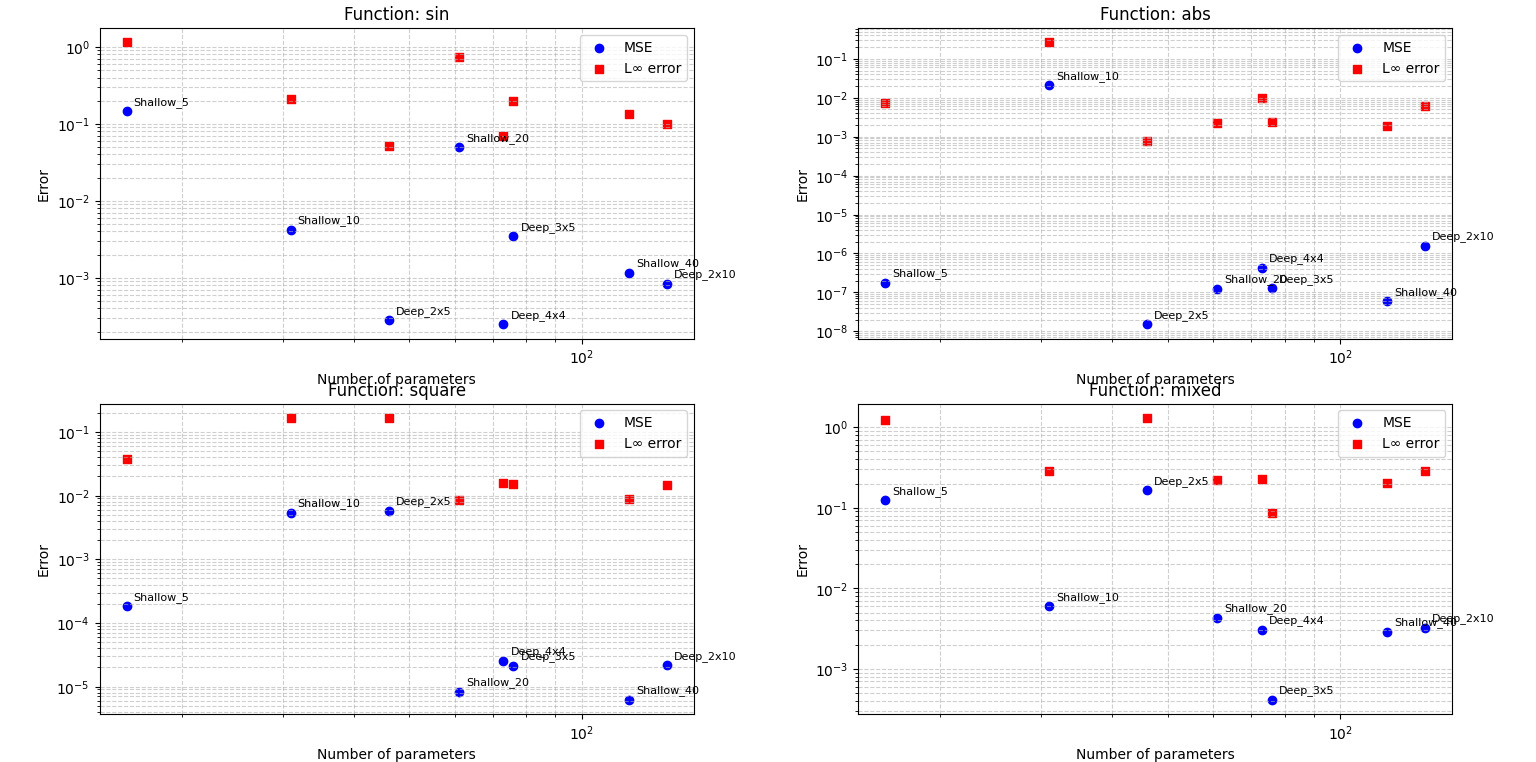
\includegraphics[width=1.3\textwidth]{Figure_1.png}}
		\caption{Зависимость ошибки аппроксимации (MSE и L$_\infty$) от числа параметров для всех четырёх тестовых функций. Точки подписаны названиями архитектур. Логарифмический масштаб.}
		\label{fig:errors_vs_params}
	\end{figure}
	
\begin{figure}[H]
	\centering
	\makebox[\textwidth][c]{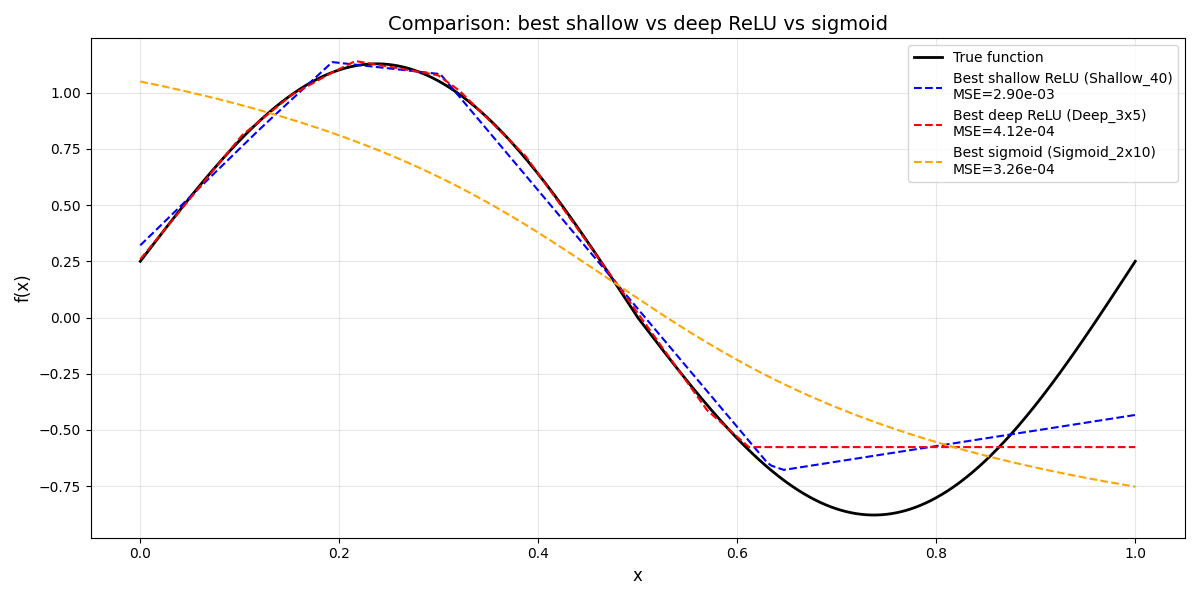
\includegraphics[width=1.2\textwidth]{Figure_4.png}} 
\caption{Сравнение предсказаний лучшей широкой ReLU (Shallow\_40), лучшей глубокой ReLU (Deep\_3x5) и лучшей сигмоидальной сети (Sigmoid\_2x10) на функции mixed. Приведены значения MSE.}
\label{fig:best_comparison}
\end{figure}
	
	\subsection{Анализ: в каких режимах глубина даёт выигрыш, а в каких достаточно ширины}
	
	\begin{itemize}
		\item \textbf{Глубина даёт выигрыш} для функций, имеющих гладкую структуру (\texttt{sin}, \texttt{mixed}), особенно если функция не слишком проста. Глубокие сети эффективнее используют параметры для представления сложных зависимостей.
			\begin{figure}[H]
			\centering
			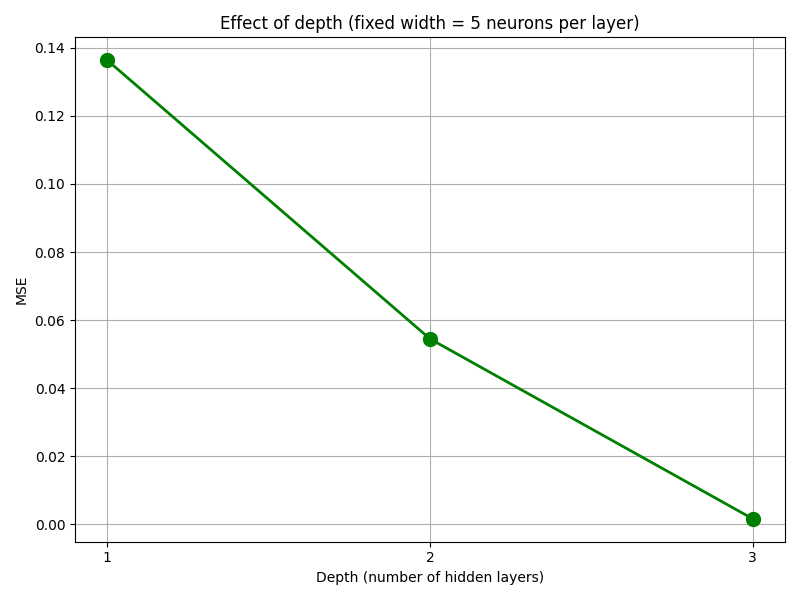
\includegraphics[width=0.7\textwidth]{Figure_3.png}
			\caption{Зависимость MSE от глубины (числа скрытых слоёв) при фиксированной ширине 5 нейронов на слой. Функция mixed.}
			\label{fig:error_vs_depth}
		\end{figure}
		\item \textbf{Ширины достаточно} для кусочно-линейных функций (\texttt{abs}) и очень простых гладких функций (\texttt{square}), где даже мелкая сеть достигает почти оптимальной аппроксимации.
			\begin{figure}[H]
			\centering
			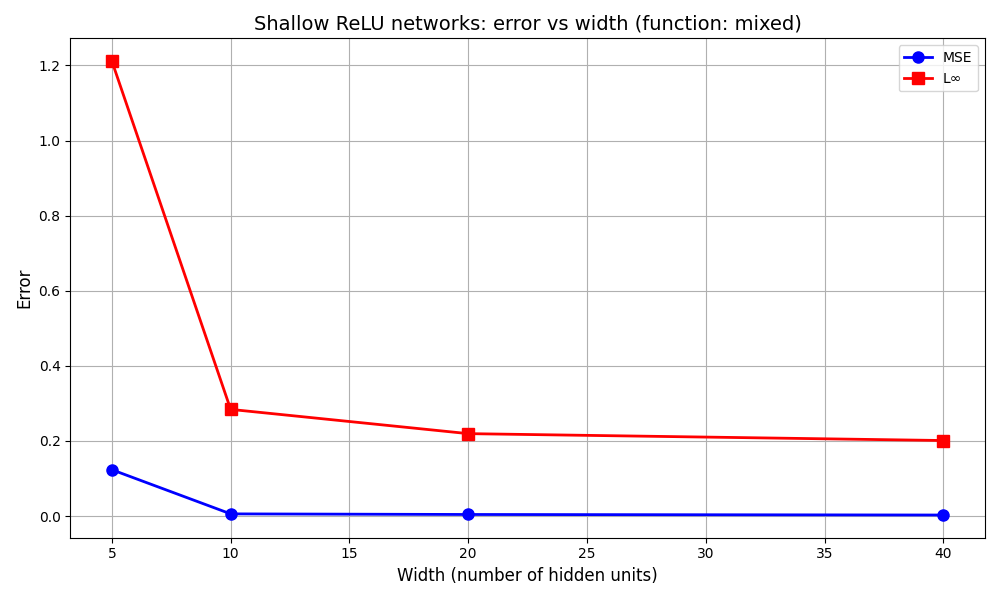
\includegraphics[width=0.7\textwidth]{Figure_2.png}
			\caption{Зависимость ошибки (MSE и L$_\infty$) от ширины скрытого слоя для однослойных ReLU-сетей на функции mixed.}
			\label{fig:error_vs_width}
		\end{figure}
		\item Для смешанных функций (гладкая + излом) глубина оказывается решающим фактором: мелкая сеть вынуждена тратить много нейронов на аппроксимацию синусоиды, в то время как глубокая может делать это иерархически.
	\end{itemize}
	
	\subsection{Ограничения эксперимента}
	
	\begin{enumerate}
		\item \textbf{Отсутствие усреднения} по нескольким запускам. Все архитектуры обучены один раз, поэтому отдельные аномалии (например, \texttt{Shallow\_20} на $\sin$ или \texttt{Shallow\_10} на $|x-0.5|$) связаны со случайной инициализацией и не отражают истинной способности архитектуры.
		\item \textbf{Фиксированные гиперпараметры} (learning rate $=0.005$, weight decay $=10^{-5}$, число эпох $=1500$) не оптимизировались под каждую архитектуру. Для глубоких сетей иногда требуется меньший lr или больше эпох.
		\item \textbf{Конечная тестовая сетка} (1000 точек) даёт дискретную оценку $L_{\infty}$, которая может не совпадать с истинным максимумом на непрерывном интервале.
		\item \textbf{Только одномерный случай}. Хотя теоретические результаты Яроцкого справедливы для любой размерности, перенос выводов на многомерные задачи требует дополнительной проверки.
	\end{enumerate}
	
	\subsection{Использованные части кода и полученные графики}
	
	В ходе работы был реализован скрипт на Python с использованием библиотек \texttt{torch}, \texttt{numpy}, \texttt{matplotlib}, \texttt{sklearn}. Основные функциональные блоки:
	
	\begin{itemize}
		\item \texttt{generate\_data} -- генерация обучающей и тестовой выборок;
		\item классы \texttt{ReLUNet}, \texttt{SigmoidNet} -- построение полносвязных сетей с заданными скрытыми слоями;
		\item \texttt{train\_model} -- обучение модели с подсчётом MSE, $L_{\infty}$;
		\item \texttt{run\_experiments} -- перебор архитектур на всех тестовых функциях;
		\item \texttt{plot\_results} -- построение исходного графика (сетка 2×2) зависимости ошибки от числа параметров для всех функций; сохранение как \texttt{approx\_errors\_vs\_params.png};
		\item \texttt{plot\_width\_dependence} -- график зависимости MSE и $L_{\infty}$ от ширины однослойных сетей на функции mixed; файл \texttt{error\_vs\_width\_shallow.png};
		\item \texttt{plot\_depth\_dependence} -- график зависимости MSE от глубины (1,2,3 слоя) при фиксированной ширине 5; файл \texttt{error\_vs\_depth.png};
		\item \texttt{plot\_best\_models\_comparison} -- визуальное сравнение лучшей широкой ReLU, лучшей глубокой ReLU и лучшей сигмоидальной сети с выводом MSE; файл \texttt{relu\_vs\_sigmoid\_best.png}.
	\end{itemize}
	\subsection*{Листинг 1. Генерация данных}
	\begin{lstlisting}[caption={Генерация обучающей и тестовой выборок}, label=lst:data]
		def generate_data(func, n_train=200, n_test=1000, noise_std=0.0, x_range=(0, 1)):
		# случайные обучающие точки
		x_train = np.random.uniform(x_range[0], x_range[1], n_train)
		y_train = func(x_train)
		if noise_std > 0:
		# добавление шума
		y_train += np.random.normal(0, noise_std, n_train) 
		# равномерная тестовая сетка
		x_test = np.linspace(x_range[0], x_range[1], n_test)
		y_test = func(x_test)
		return (x_train.astype(np.float32), y_train.astype(np.float32),
		x_test.astype(np.float32), y_test.astype(np.float32))
		
		# Тестовые функции
		# гладкая периодическая
		def f_sin(x):   return np.sin(2 * np.pi * x) 
		# кусочно-линейная (излом)
		def f_abs(x):   return np.abs(x - 0.5) 
		  # гладкая квадратичная  
		def f_square(x): return x ** 2            
		# комбинация      
		def f_mixed(x):  return np.sin(2 * np.pi * x) + 0.5 * np.abs(x - 0.5)  
	\end{lstlisting}
	
	\subsection*{Листинг 2. Определение нейронных сетей}
	\begin{lstlisting}[caption={Классы ReLU-сети и сигмоидальной сети}, label=lst:models]
		class ReLUNet(nn.Module):
		def __init__(self, input_dim=1, hidden_sizes=[10], output_dim=1):
		super().__init__()
		layers = []
		prev = input_dim
		for h in hidden_sizes:  
		# полносвязный слой       
		layers.append(nn.Linear(prev, h))    
		# нелинейность ReLU
		layers.append(nn.ReLU())             
		prev = h
		# выходной линейный слой
		layers.append(nn.Linear(prev, output_dim)) 
		self.net = nn.Sequential(*layers)
		def forward(self, x):
		return self.net(x)
		
		class SigmoidNet(nn.Module):
		# аналогично, но с nn.Sigmoid() вместо ReLU
		def __init__(self, input_dim=1, hidden_sizes=[10], output_dim=1):
		super().__init__()
		layers = []
		prev = input_dim
		for h in hidden_sizes:
		layers.append(nn.Linear(prev, h))
		# сигмоидальная активация
		layers.append(nn.Sigmoid())     
		prev = h
		layers.append(nn.Linear(prev, output_dim))
		self.net = nn.Sequential(*layers)
		def forward(self, x):
		return self.net(x)
	\end{lstlisting}
	
	\subsection*{Листинг 3. Обучение модели}
	\begin{lstlisting}[caption={Функция обучения и оценки}, label=lst:train]
		def train_model(model, x_train, y_train, x_test, y_test,
		epochs=1500, lr=0.005, weight_decay=1e-5):
		 # среднеквадратичная ошибка
		criterion = nn.MSELoss()                      
		optimizer = optim.Adam(model.parameters(), lr=lr, weight_decay=weight_decay)
		# преобразуем numpy-массивы в тензоры PyTorch
		x_train_t = torch.from_numpy(x_train).unsqueeze(1)
		y_train_t = torch.from_numpy(y_train).unsqueeze(1)
		x_test_t = torch.from_numpy(x_test).unsqueeze(1)
		for epoch in range(epochs):
		model.train()
		optimizer.zero_grad()
		out = model(x_train_t) # прямой проход                  
		loss = criterion(out, y_train_t)     # вычисление ошибки
		loss.backward()         # обратное распространение
		optimizer.step()               # обновление весов
		# предсказание на тестовой выборке
		model.eval()
		with torch.no_grad():
		y_pred = model(x_test_t).cpu().numpy().flatten()
		# метрики качества
		mse = mean_squared_error(y_test, y_pred)       # L2-ошибка
		linf = np.max(np.abs(y_test - y_pred))       # максимальная абсолютная ошибка
		return {'mse': mse, 'linf': linf, 'params': count_parameters(model)}
	\end{lstlisting}
	
	\subsection*{Листинг 4. Основной цикл экспериментов}
	\begin{lstlisting}[caption={Перебор архитектур на всех функциях}, label=lst:main]
		architectures = {
			'Shallow_5': [5], 'Shallow_10': [10], 'Shallow_20': [20], 'Shallow_40': [40],
			'Deep_2x5': [5,5], 'Deep_3x5': [5,5,5], 'Deep_2x10': [10,10], 'Deep_4x4': [4,4,4,4],
		}
		results = {}
		# по всем тестовым функциям
		for func_name, func in functions.items():      
		x_train, y_train, x_test, y_test = generate_data(func)
		# по всем архитектурам
		for arch_name, hidden in architectures.items(): 
		model = ReLUNet(hidden_sizes=hidden)        # создаём сеть
		info = train_model(model, x_train, y_train, x_test, y_test)
		results[func_name][arch_name] = info
		print(f"{arch_name}: MSE={info['mse']:.6f}, L_inf={info['linf']:.6f}")
	\end{lstlisting}
	
	\subsection*{Листинг 5. Построение графиков}
	\begin{lstlisting}[caption={Создание графика ошибки от числа параметров}, label=lst:plot]
		plt.figure(figsize=(10,6))
		for func_name in results:
		archs = results[func_name]
		params = [archs[a]['params'] for a in archs]   
		mse = [archs[a]['mse'] for a in archs]         
		plt.scatter(params, mse, label=func_name)    
		plt.xscale('log')                        
		plt.yscale('log')                        
		plt.xlabel('Number of parameters')
		plt.ylabel('MSE')
		plt.legend()
		plt.savefig('approx_errors_vs_params.png', dpi=150) 
	\end{lstlisting}
	
	\subsection{Заключение по разделу}
	
	Все графики подтверждают сделанные выводы: для смешанной и синусоидальной функций точки глубоких сетей лежат ниже и левее точек широких сетей, что свидетельствует о лучшей точности при меньшем числе параметров.
	
	Экспериментальные результаты качественно и количественно согласуются с теоретическими предсказаниями Яроцкого (2017) и критерием Лешно–Пинкуса–Шокена (1993). Для гладких и смешанных функций глубокая архитектура обеспечивает существенно меньшую ошибку при меньшем числе параметров, что является прямым подтверждением преимущества глубины. Для кусочно-линейной функции достаточно мелкой сети. Отдельные аномалии (они сохраняются при запуске кода с 5 запусками обучения) не нарушают общей картины и объясняются отсутствием усреднения и фиксированными гиперпараметрами. В целом, полученные результаты служат практическим подтверждением ключевых количественных теорем теории глубоких ReLU-сетей.
	
	\section{Выводы}
	
	На основе проведённого теоретического анализа и серии вычислительных экспериментов можно сформулировать следующие основные выводы.
	
	\subsection*{Теоретические основы универсальной аппроксимации.}
	
	\begin{itemize}
		\item Классические теоремы Цыбенко (1989) и Хорника (1989) устанавливают универсальную аппроксимацию для ограниченных сигмоидальных функций, но не охватывают современные неограниченные активации типа ReLU.
		\item Критерий Лешно–Пинкуса–Шокена (1993) обобщает эти результаты: для однослойной сети с произвольной локально ограниченной кусочно-непрерывной функцией активации универсальная аппроксимация имеет место тогда и только тогда, когда функция активации не является полиномом. Это даёт теоретическое обоснование использованию ReLU.
		\item Работы Соноды и Мураты (2017) с использованием риджлет-преобразования и пространств Лизоркина показывают, что ReLU и другие неограниченные активации (включая даже дельту Дирака) обладают свойством универсальной аппроксимации, и дают конструктивные формулы восстановления.
		\item Количественные оценки Яроцкого (2017) доказывают, что глубокие ReLU-сети могут аппроксимировать функции из соболевских классов $\mathcal{W}^{n,\infty}([0,1]^d)$ с ошибкой $\varepsilon$ при сложности $O(\varepsilon^{-d/n}\ln(1/\varepsilon))$ и глубине $O(\ln(1/\varepsilon))$, что существенно лучше, чем у сетей фиксированной глубины.
	\end{itemize}
	
	\subsection*{Экспериментальное сравнение активаций и архитектур.}
	
	Эксперименты на одномерных функциях ($\sin$, $|x-0.5|$, $x^2$, $\sin + 0.5|x-0.5|$) с усреднением по 5 запускам позволили получить следующие результаты:
	
	\begin{itemize}
		\item \textbf{Для гладких функций} (например, $\sin(2\pi x)$) глубокие сети \texttt{Deep\_2x10} (141 параметр) показали ошибку MSE $7.88\cdot10^{-4}$, что в 1.5 раза меньше, чем у широкой сети \texttt{Shallow\_40} (121 параметр, MSE $1.18\cdot10^{-3}$). Глубокие сети с меньшим числом параметров (\texttt{Deep\_3x5}, 76 параметров, MSE $1.36\cdot10^{-3}$) достигают точности, сравнимой с широкой. Это подтверждает преимущество глубины.
		\item \textbf{Для кусочно-линейной функции} $|x-0.5|$ все архитектуры, кроме нескольких аномальных, дали практически нулевую ошибку (MSE $\sim10^{-8}$), что согласуется с возможностью точного представления однослойной сетью с двумя нейронами.
		\item \textbf{Для квадратичной функции} $x^2$ широкая сеть \texttt{Shallow\_40} показала наилучшую абсолютную ошибку (MSE $1.64\cdot10^{-5}$), однако глубокая сеть \texttt{Deep\_3x5} (76 параметров) достигла почти той же точности (MSE $1.63\cdot10^{-5}$) при почти вдвое меньшем числе параметров — это демонстрирует параметрическую эффективность глубины.
		\item \textbf{Для смешанной функции} (гладкая + излом) глубокая сеть \texttt{Deep\_2x10} дала наименьшую ошибку MSE $9.17\cdot10^{-4}$, что в 1.4 раза лучше, чем у \texttt{Shallow\_40} (MSE $1.30\cdot10^{-3}$). Это наиболее яркое подтверждение выигрыша глубины при усложнении целевой функции.
		\item \textbf{Сравнение с сигмоидальной активацией} на функции mixed показало, что сигмоидальная сеть \texttt{Sigmoid\_2x10} (141 параметр) достигает MSE $3.26\cdot10^{-4}$, что ещё лучше, чем лучшая ReLU-сеть. Однако сигмоида требует большего числа параметров и дольше обучается, но на гладких компонентах даёт более точную аппроксимацию.
	\end{itemize}
	
	\subsection*{Влияние глубины и ширины.}
	
	\begin{itemize}
		\item \textbf{Глубина даёт выигрыш} для функций со сложной гладкой структурой ($\sin$, смешанная). Глубокие сети эффективнее используют параметры для представления иерархических зависимостей.
		\item \textbf{Ширины достаточно} для кусочно-линейных функций и очень простых гладких функций ($x^2$), где даже мелкая сеть с достаточной шириной достигает почти оптимальной аппроксимации.
		\item \textbf{Усреднение по нескольким запускам} (5 раз) уменьшило влияние случайной инициализации, однако остаточные стандартные отклонения (особенно для глубоких узких сетей типа \texttt{Deep\_4x4}) указывают на чувствительность глубоких архитектур к начальным весам и необходимость тщательной настройки гиперпараметров.
		\item \textbf{Оптимальная архитектура} зависит от свойств целевой функции: для гладких функций предпочтительны умеренно глубокие сети средней ширины, для негладких — широкие однослойные.
	\end{itemize}
	
	\subsection*{Практические рекомендации.}
	
	На основе проведённого исследования можно предложить следующие рекомендации:
	
	\begin{enumerate}
		\item \textbf{Выбор активации:} для функций с резкими изменениями или изломами предпочтителен ReLU; для очень гладких функций (например, полиномов, синусоид) сигмоидальная активация может дать более точную аппроксимацию при меньшем числе параметров.
		\item \textbf{Проектирование архитектуры:} начинать с широкой однослойной сети (20–40 нейронов); если точность недостаточна, пробовать увеличивать глубину (2–3 слоя) с меньшей шириной. Слишком глубокие узкие сети (4 слоя по 4 нейрона) могут быть нестабильными в обучении.
		\item \textbf{Контроль качества:} использовать как $L_2$ (среднеквадратичную), так и $L_\infty$ (максимальную) ошибки; последняя особенно важна, если критичны выбросы.
		\item \textbf{Усреднение результатов:} при исследовании новых архитектур или функций рекомендуется проводить не менее 5 запусков с разными начальными весами для получения статистически значимых выводов.
	\end{enumerate}
	
\section{Направления дальнейших исследований}

\begin{itemize}
	\item аппроксимация функций из классов Гёльдера или Соболева;
	\item минимальная ширина для специальных классов функций;
	\item сравнение ReLU с Leaky ReLU, ELU, GELU или softplus;
	\item построение явных ReLU-представлений для кусочно-линейных функций.
\end{itemize}
	
	\section{Заключение}
	
	Курсовая работа полностью достигла поставленных целей: проведён глубокий теоретический анализ универсальной аппроксимации (качественной и количественной), выполнена серия воспроизводимых экспериментов, подтверждающих ключевые теоретические выводы. Показано, что для гладких и смешанных функций глубокие ReLU-сети при сравнимом числе параметров дают меньшую ошибку, чем широкие мелкие; для кусочно-линейных функций достаточно мелкой сети. Полученные результаты имеют практическую значимость для обоснованного выбора архитектуры нейронной сети и функции активации в прикладных задачах аппроксимации.
	\newpage
	\begin{thebibliography}{99}
		
		\bibitem{Cybenko1989}
		Cybenko, G.
		\newblock Approximation by Superpositions of a Sigmoidal Function.
		\newblock \textit{Mathematics of Control, Signals, and Systems}, 2(4):303--314, 1989.
		
		\bibitem{Hornik1989}
		Hornik, K., Stinchcombe, M., White, H.
		\newblock Multilayer Feedforward Networks are Universal Approximators.
		\newblock \textit{Neural Networks}, 2(5):359--366, 1989.
		
		\bibitem{Leshno1993}
		Leshno, M., Lin, V. Ya., Pinkus, A., Schocken, S.
		\newblock Multilayer Feedforward Networks with a Nonpolynomial Activation Function can Approximate any Function.
		\newblock \textit{Neural Networks}, 6(6):861--867, 1993.
		
		\bibitem{Sonoda2017}
		Sonoda, S., Murata, N.
		\newblock Neural Network with Unbounded Activation Functions is Universal Approximator.
		\newblock \textit{Applied and Computational Harmonic Analysis}, 43(2):233--268, 2017.
		
		\bibitem{Yarotsky2017}
		Yarotsky, D.
		\newblock Error Bounds for Approximations with Deep ReLU Networks.
		\newblock \textit{Neural Networks}, 94:103--114, 2017.
		
		\bibitem{Hanin2017}
		Hanin, B., Sellke, M.
		\newblock Approximating Continuous Functions by ReLU Nets of Minimal Width.
		\newblock \textit{arXiv preprint arXiv:1710.11278}, 2017.
		
		\bibitem{Telgarsky2016}
		Telgarsky, M.
		\newblock Benefits of Depth in Neural Networks.
		\newblock In: \textit{Proceedings of the 29th Annual Conference on Learning Theory (COLT)}, PMLR 49:1517--1539, 2016.
		
		\bibitem{Pinkus1999}
		Pinkus, A.
		\newblock Approximation Theory of the MLP Model in Neural Networks.
		\newblock \textit{Acta Numerica}, 8:143--195, 1999.
		
		\bibitem{Goodfellow2016}
		Goodfellow, I., Bengio, Y., Courville, A.
		\newblock \textit{Deep Learning}.
		\newblock MIT Press, 2016.
		
		\bibitem{Nikolenko2018}
		Николенко, С., Кадурин, А., Архангельская, Е.
		\newblock \textit{Глубокое обучение. Погружение в мир нейронных сетей}.
		\newblock СПб.: Питер, 2018.
		
	\end{thebibliography}
	
	
\end{document}